\documentclass[border=3pt]{standalone}
% Preâmbulo compartilhado pelos diagramas TikZ da aula 4 de Navegação (Representação de Mapas)
\usepackage[T1]{fontenc}
\usepackage[utf8]{inputenc}
\usepackage{lmodern}
\usepackage{amsmath}
\usepackage{xcolor}
\usepackage{tikz}
\usetikzlibrary{arrows.meta,angles,quotes,decorations.pathmorphing,decorations.pathreplacing,calc,
                positioning,shapes.geometric,shapes.misc,backgrounds,fit,
                math}

% Paleta (mesma dos SVGs originais)
\definecolor{dblue}{HTML}{2A5B8C}
\definecolor{dorange}{HTML}{B3541E}
\definecolor{dgreen}{HTML}{4A7C59}
\definecolor{dred}{HTML}{9C4B4B}
\definecolor{dcream}{HTML}{F4F1EA}
\definecolor{dshade}{HTML}{DDD7C9}

% Função gaussiana (não normalizada por padrão de escala visual)
\pgfmathdeclarefunction{gauss}{3}{%
  \pgfmathparse{1/(#3*sqrt(2*pi))*exp(-((#1-#2)^2)/(2*#3^2))}%
}

% Estilos comuns (prefixo d... para não colidir com chaves internas do pgf)
\tikzset{
  >={Stealth[length=2mm]},
  dguide/.style={gray!55, dashed, line width=0.4pt},
  daxis/.style={gray!60, line width=0.7pt, ->},
  dbody/.style={fill=black!3, draw=black!80, line width=1pt},
  dacc/.style={draw=dblue, line width=1pt},
  dlbl/.style={black!55, font=\small},
  dsub/.style={black!45, font=\footnotesize},
  dstate/.style={circle, draw=black!80, fill=dcream, line width=1pt,
                 minimum size=17mm, font=\large, inner sep=1pt},
  dobs/.style={circle, draw=black!80, fill=dshade, line width=1pt,
               minimum size=14mm, font=\large, inner sep=1pt},
  dbox/.style={rounded corners=2pt, draw=black!80, fill=dcream, line width=1pt,
               align=center, inner sep=6pt},
  dop/.style={circle, draw=black!80, fill=white, line width=1pt,
              minimum size=6mm, inner sep=0pt, font=\small},
  dtrans/.style={->, dblue, line width=1pt},
  dmeas/.style={->, dorange, line width=1pt},
  dcurve/.style={line width=1pt, dblue},
  dcurveb/.style={line width=1.4pt, dorange},
}

\begin{document}
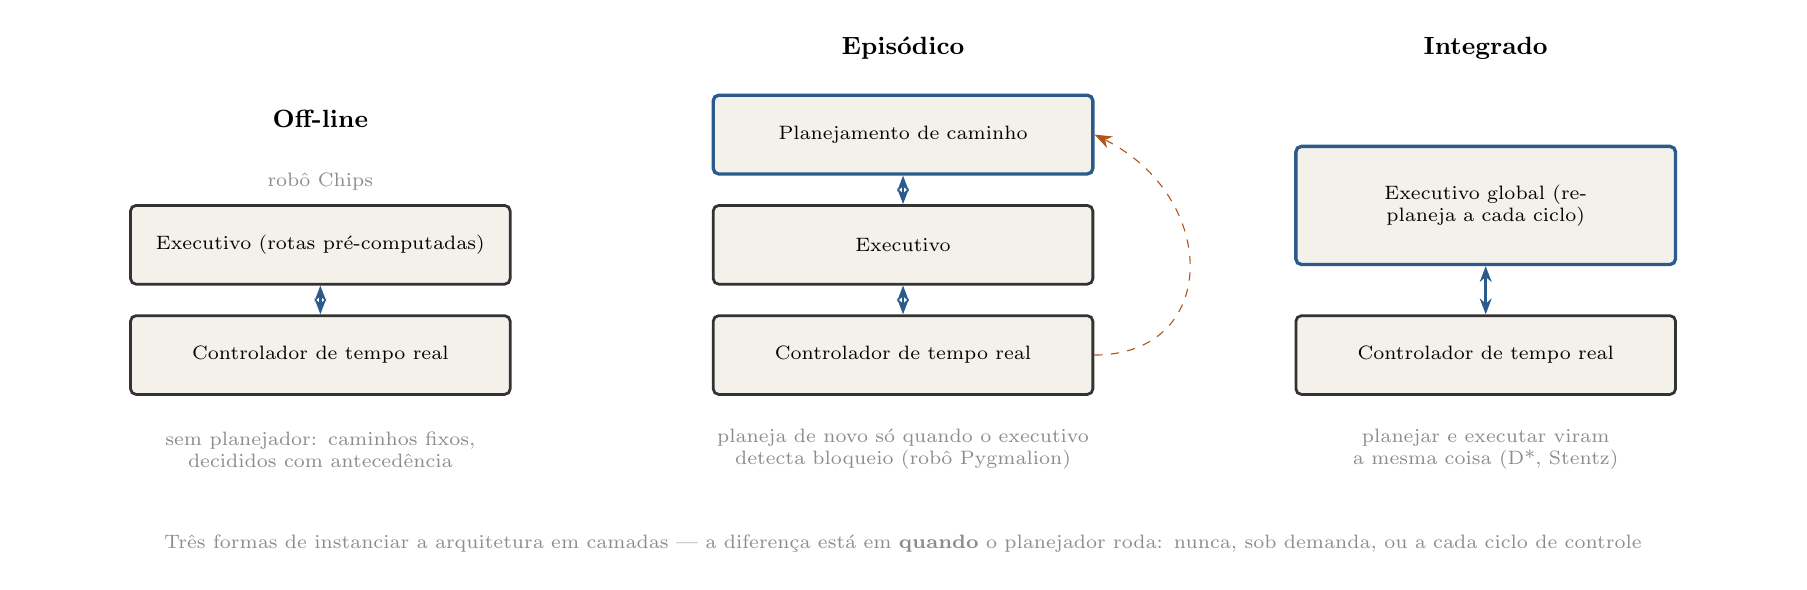
\begin{tikzpicture}[x=1cm,y=1cm]

  % Painel A: off-line (Chips)
  \begin{scope}[shift={(0,0)}]
    \node[dbox, text width=4.4cm, font=\scriptsize, minimum height=1.0cm] (ex) at (0,1.4) {Executivo (rotas pré-computadas)};
    \node[dbox, text width=4.4cm, font=\scriptsize, minimum height=1.0cm] (rt) at (0,0) {Controlador de tempo real};
    \draw[dtrans, <->] (ex.south) -- (rt.north);
    \node[font=\bfseries\small] at (0,3.0) {Off-line};
    \node[dsub, font=\scriptsize] at (0,2.2) {robô Chips};
    \node[dsub, font=\scriptsize, align=center, text width=5.4cm] at (0,-1.2)
       {sem planejador: caminhos fixos, decididos com antecedência};
  \end{scope}

  % Painel B: episódico (Pygmalion)
  \begin{scope}[shift={(7.4,0)}]
    \node[dbox, text width=4.4cm, font=\scriptsize, minimum height=1.0cm, draw=dblue, line width=1.2pt] (pp) at (0,2.8) {Planejamento de caminho};
    \node[dbox, text width=4.4cm, font=\scriptsize, minimum height=1.0cm] (ex) at (0,1.4) {Executivo};
    \node[dbox, text width=4.4cm, font=\scriptsize, minimum height=1.0cm] (rt) at (0,0) {Controlador de tempo real};
    \draw[dtrans, <->] (ex.south) -- (rt.north);
    \draw[dtrans, <->] (pp.south) -- (ex.north);
    \draw[dorange, dashed, -{Stealth[length=2.2mm]}] (rt.east) .. controls +(1.6,0) and +(1.6,-0.8) .. (pp.east);
    \node[font=\bfseries\small] at (0,3.9) {Episódico};
    \node[dsub, font=\scriptsize, align=center, text width=5.4cm] at (0,-1.2)
       {planeja de novo só quando o executivo detecta bloqueio (robô Pygmalion)};
  \end{scope}

  % Painel C: integrado (D*)
  \begin{scope}[shift={(14.8,0)}]
    \node[dbox, text width=4.4cm, font=\scriptsize, minimum height=1.5cm, draw=dblue, line width=1.2pt] (ge) at (0,1.9) {Executivo global (replaneja a cada ciclo)};
    \node[dbox, text width=4.4cm, font=\scriptsize, minimum height=1.0cm] (rt) at (0,0) {Controlador de tempo real};
    \draw[dtrans, <->] (ge.south) -- (rt.north);
    \node[font=\bfseries\small] at (0,3.9) {Integrado};
    \node[dsub, font=\scriptsize, align=center, text width=5.4cm] at (0,-1.2)
       {planejar e executar viram a mesma coisa (D*, Stentz)};
  \end{scope}

  \node[dsub, font=\scriptsize, align=center, text width=22cm] at (7.4,-2.4)
     {Três formas de instanciar a arquitetura em camadas --- a diferença está em \textbf{quando} o planejador roda: nunca, sob demanda, ou a cada ciclo de controle};

\end{tikzpicture}
\end{document}
